
\documentclass[12pt]{article}
\pagestyle{empty} \topmargin -0.5in \textheight 9in \textwidth 6.5in
\oddsidemargin -0in
\usepackage{amssymb}
\usepackage{amsmath}
\usepackage{xcolor}
\usepackage{graphicx}
\usepackage[normalem]{ulem}
\usepackage{enumerate}

\DeclareMathOperator{\tr}{tr}

\newcommand{\vect}[1]{\mathbf{#1}}

\begin{document}

\begin{flushleft}

\textbf{Department of Applied Mathematics and Statistics}

\textbf{COLORADO SCHOOL OF MINES}\\


MATH $455$: Partial Differential Equations
\end{flushleft}

\vspace{0.1in}

\begin{center}
{\bf Assignment \#1 - Fourier Series} \\
Due Tuesday, September 8, 2026 \\
\end{center}

\vspace{0.3in}

\noindent $\textbf{1}$. (15 points) Let $f$ be a $2\pi$-periodic function satisfying $f(x) = x$ for $x \in (-\pi, \pi)$. 
\begin{enumerate}[(a)]
\item Compute the Fourier series of $f$ and show all work. \\ \\
\textcolor{blue}{\textbf{Solution} — The Fourier series of a periodic function $f(x)$ over the domain of one period $[a,b]$ is given by $$f(x) = \frac{1}{2} a_0 + \sum_{n=1}^{\infty} a_n \cos(nx) + \sum_{n=1}^{\infty} b_n \sin(nx)$$ where $$a_0 = \frac{2}{b - a} \int_a^b f(x)dx \;\;\;\;\;\;\;a_n = \frac{2}{b-a} \int_a^b f(x)\cos(nx) dx$$ \\ $$b_n = \frac{2}{b-a} \int_a^b f(x) \sin(nx) dx$$ \\ \\ 
Then for our specific $2\pi$-periodic function $f(x) = x$, we have $$a_0  = \frac{1}{\pi} \int_{-\pi}^{\pi} x dx = 0 \;\; \text{(by oddness)}$$ $$a_n = \frac{1}{\pi} \int_{-\pi}^{\pi} x \cos(nx) dx = 0 \;\; \text{(also by oddness)}$$
\begin{align*}
b_n &= \frac{1}{\pi} \int_{-\pi}^{\pi} x \sin(nx)dx \\
&= \frac{2}{\pi} \int_0^{\pi} x \sin(nx) dx \;\; \text{(by evenness)} \\
&= \frac{2}{\pi} \left[ \frac{-x}{n}  \left. \cos(nx) \right|_{0}^{\pi} + \frac{1}{n} \int_0^{\pi} \cos(nx)dx   \right] \;\; \text{(by IBP)} \\
&= \frac{2}{\pi} \left[ \frac{-\pi}{n} \cos(nx) + \frac{\sin(n\pi)}{n^2}   \right]  \\
&= \frac{2\sin(n\pi)}{\pi n^2} - \frac{2}{n} \cos(nx)  \\
\end{align*}
Thus our series expansion is $$f(x) = \sum_{n=1}^{\infty} \left[ \frac{2\sin(n\pi)}{\pi n^2} - \frac{2}{n} \cos(nx) \right] \sin(nx)$$ Note that $\sin(n\pi) = 0$ and $\cos(n\pi) = (-1)^{n}$ for $n=1,2,3 \cdots$. Hence, we have $$\boxed{f(x) = 2\sum_{n=1}^{\infty} \frac{(-1)^{n+1} \sin(nx)}{n}}$$ 
}
\item Using your answer from (a), graph by hand on the same axes the three functions $f(x), g(x)$, and $h(x)$ on the interval $[-\pi,\pi]$  where
$$ g(x) = b_1 \sin(x)$$
and
$$ h(x) = b_1 \sin(x) + b_2 \sin(2x)$$
are the one-term and two-term Fourier Series approximations of $f$, respectively. \\ \\
\textcolor{blue}{\textbf{Solution} —We have $g(x) = 2\sin(x)$ and $h(x) = 2\sin(x) - \sin(2x)$} \\ \\
\begin{figure}[h]
    \centering 
    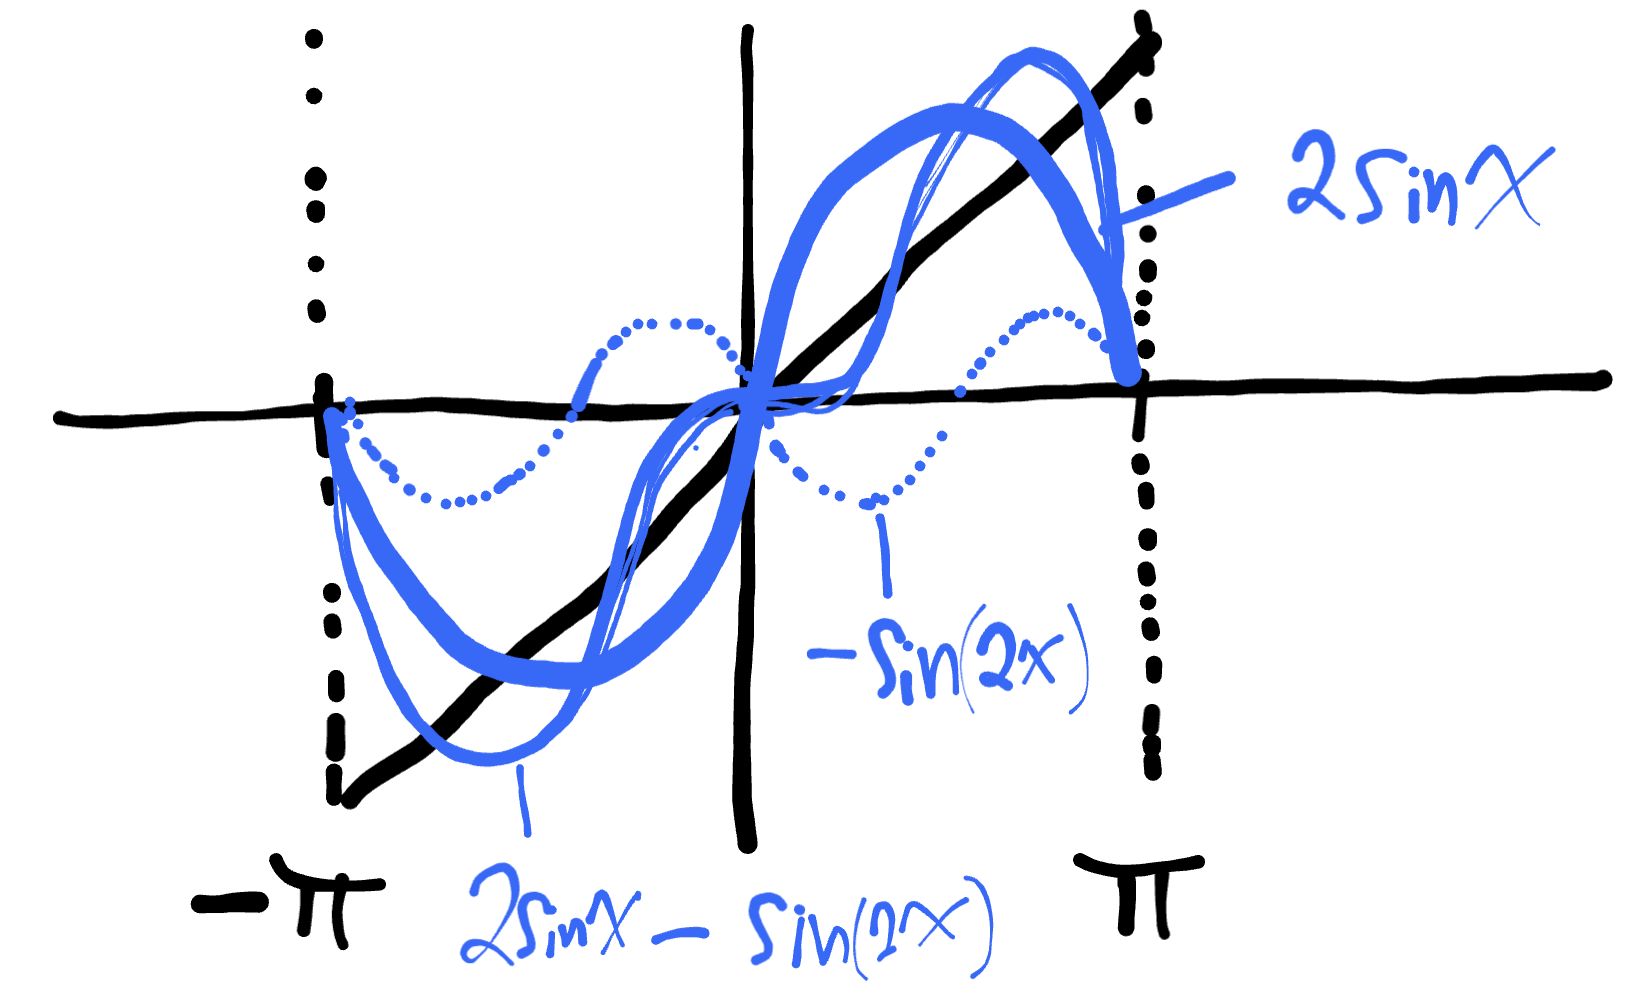
\includegraphics[width=0.5\textwidth]{1}
\end{figure}
\end{enumerate}


\vspace{0.3in}

\noindent $\textbf{2}$. (5 points) Let $f(x)$ be a given function for $x \in [-\pi, \pi]$ and find $c \in \mathbb{R}$ which minimizes
$$\int_{-\pi}^\pi \left ( f(x) - c \right )^2 \ dx.$$
Note that your answer should depend in some manner upon the given function $f$.\\ \\
\textcolor{blue}{\textbf{Solution} — Let us find the $c$ that minimizes 
\begin{align*}
D(c) &= \int_{-\pi}^{\pi} (f(x) - c)^2
\end{align*}
Note that $D(c)$ appears to be some of sort of distance-squared metric measuring the accumulated distance between $f(x)$ and the line $y=c$. So intuitively, we expect $c$ has to be something like the average value of $f(x)$ in order for all of $f$ to be as close as possible to $c$—that is, to minimize this distance. We will use the first derivative test.  $$\frac{dD}{dc} = \frac{d}{dc} \int_{-\pi}^{\pi} (f(x) - c)^2 dx$$ We can bring the derivative inside the integral because it is independent of the variable of integration $x$. Doing this will translate the derivative into a partial derivative, because the integrand is a function of both $x$ and the parameter $c$.
\begin{align*}
&=  \int_{-\pi}^{\pi} \frac{\partial}{\partial c} (f(x) - c)^2 dx \\
&=   \int_{-\pi}^{\pi} 2 (f(x) - c)(0 - 1) dx \\
&=   2 \int_{-\pi}^{\pi} (c - f(x)) dx \\
&=   4\pi c - 2 \int_{-\pi}^{\pi} f(x) dx = 0 \\
&\implies \boxed{c = \frac{1}{2\pi} \int_{-\pi}^{\pi} f(x) dx} 
\end{align*}
So the value of $c$ that minimizes $D(c)$ happens to be exactly the average value of $f(x)$ over $[-\pi, \pi]$, as predicted.
}


\vspace{0.3in}


\noindent $\textbf{3}$. (10 points) Let $f(x)$ be a given function for $x \in [-\pi, \pi]$ and find $a, b, c \in \mathbb{R}$ which minimize
$$\int_{-\pi}^\pi \left ( f(x) - a\cos(x) - b\sin(x) - c \right )^2 \ dx.$$
Again, note that your answer should depend in some manner upon the given function $f$ and use the analogous hint as above for a multivariate function.\\ \\
\textcolor{blue}{\textbf{Solution} — Let $$F(a,b,c) = \int_{-\pi}^\pi \left ( f(x) - a\cos(x) - b\sin(x) - c \right )^2 \ dx$$ \\ Then we would like to minimize $F$. We find where the gradient of $F$ is zero: \\
\begin{align*}
\nabla F(a,b,c) = \left\langle \frac{\partial F}{\partial a}, \frac{\partial F}{\partial b}, \frac{\partial F}{\partial c} \right\rangle = \mathbf{0}
\end{align*}
\begin{align*}
\frac{\partial F}{\partial a} &= \frac{\partial}{\partial a} \int_{-\pi}^\pi \left ( f(x) - a\cos(x) - b\sin(x) - c \right )^2 \ dx \\
&= \int_{-\pi}^\pi  2( f(x) - a\cos(x) - b\sin(x) - c)(-\cos(x)) \ dx \\
&= 2 \left[-\int_{-\pi}^\pi  f(x)\cos(x) dx + a \int_{-\pi}^\pi  \cos^2(x) dx + b \int_{-\pi}^\pi  \sin(x)\cos(x) dx + c \int_{-\pi}^\pi  \cos(x) dx \right] \\
&= 2 \left[-\int_{-\pi}^\pi  f(x)\cos(x) dx + \pi a + 0 + 0 \right] = 0 \\
&\implies a = \frac{1}{\pi} \int_{-\pi}^\pi  f(x)\cos(x) dx  \\
\end{align*}
\begin{align*}
\frac{\partial F}{\partial b} &= \frac{\partial}{\partial b} \int_{-\pi}^\pi \left ( f(x) - a\cos(x) - b\sin(x) - c \right )^2 \ dx \\
&= \int_{-\pi}^\pi  2( f(x) - a\cos(x) - b\sin(x) - c)(-\sin(x)) \ dx \\
&= 2 \left[-\int_{-\pi}^\pi  f(x)\sin(x) dx + a \int_{-\pi}^\pi  \sin(x)\cos(x) dx + b \int_{-\pi}^\pi  \sin^2(x) dx + c \int_{-\pi}^\pi  \sin(x) dx \right] \\
&= 2 \left[-\int_{-\pi}^\pi  f(x)\sin(x) dx + 0 + \pi a + 0 \right] = 0 \\
&\implies b = \frac{1}{\pi} \int_{-\pi}^\pi  f(x)\sin(x) dx  \\
\end{align*}
\begin{align*}
\frac{\partial F}{\partial c} &= \frac{\partial}{\partial c} \int_{-\pi}^\pi \left ( f(x) - a\cos(x) - b\sin(x) - c \right )^2 \ dx \\
&= \int_{-\pi}^\pi  2( f(x) - a\cos(x) - b\sin(x) - c)(-1) \ dx \\
&= 2 \left[-\int_{-\pi}^\pi  f(x) dx + a \int_{-\pi}^\pi \cos(x) dx + b \int_{-\pi}^\pi  \sin(x) dx + c \int_{-\pi}^\pi dx \right] \\
&= 2 \left[-\int_{-\pi}^\pi  f(x) dx + 0 + 0 + 2\pi c \right] = 0 \\
&\implies c = \frac{1}{2\pi} \int_{-\pi}^\pi  f(x)\sin(x) dx  \\
\end{align*}
A triplet that minimizes $F$ is thus $(a,b,c) = (a_1, b_1, f_{avg})$, where $a_1$ is the first Fourier coefficient, $a_2$ is the second Fourier coefficient, and $f_{avg}$ is the average value of $f(x)$ over $[-\pi, \pi]$. We can make a rudimentary argument for why such $(a,b,c)$ is the global minimum: in order for the squared difference error between $f(x)$ and $g(x) = a \cos(x) + b\sin(x) + c$ to be minimized, $g(x)$ has to be an accurate approximation for $f(x)$, which is attained, for instance, from the first-order Fourier approximation of $f$. Changing $g(x)$ in any way results in increasing error, where $g(x)$ becomes a poorer approximation of $f$, causing squared error to increase in all such directions. Hence we have found the minimum such $(a,b,c)$.
}



\end{document}
